%\chapter{Integration}

\newcommand{\notationdetails}{(see \chref{ch:prov} for semantics of notation and \appendixsecref{appendixsec:SportSymbols} for symbols)}

\chapter{A Platform for Spatio-Temporal Sport Analysis}
\label{ch:integration}
\startchapternobreak
% Alternative names: Pipeline, Demonstration, Application, Case Study, Tool, Platform
%An integrated platform
%Case Study

% Case Studies for Software Engineers: https://ieeexplore.ieee.org/stamp/stamp.jsp?arnumber=1317512
% Case study: extreme programming in a university environment. https://dl.acm.org/citation.cfm?id=381536
% An empirical study of communication in code inspections. https://dl.acm.org/citation.cfm?doid=253228.253248
% From examples, case study, in context of software engineering, simply appears to be an observational study of an internal culture. This can lead to hypotheses generation as input to later formal studies.

% \nb{Adapted from thesis abstract}

%\vspace{5cm}

The previous chapters highlighted the need for data provenance in sport (Chapter~\ref{ch:prov}), systematically selected a means to de-identify the GPS data to protect individual privacy (Chapter~\ref{ch:de-identification}), and developed a technique to semi-automate the choice of coordinate systems at each venue to facilitate comparisons across different fields (Chapter~\ref{ch:spat-trans}). This chapter integrates the techniques proposed in the previous chapters to construct a computational pipeline for \afl{} analysis, and demonstrates that when combined they provide meaningful team-level insights without compromising individual privacy.

%\vspace{3cm}

\section{Pipeline}
%(Describe using W3C PROV notation? (generate from XML description?))


%\subsection{Overview}
%\figref{fig:digital-prov-thesis} shows the overall pipeline that will be demonstrated in this chapter (see \chref{ch:prov} for details of the custom notation used). % TODO: Highlight where work from each of the chapters appears within the diagram.

This section describes the overall pipeline constructed to support analysis of \afl{} data. See \chref{ch:prov} for details of the visual notation used to describe the pipeline.

% \begin{figure}[htbp]
% \centering
% 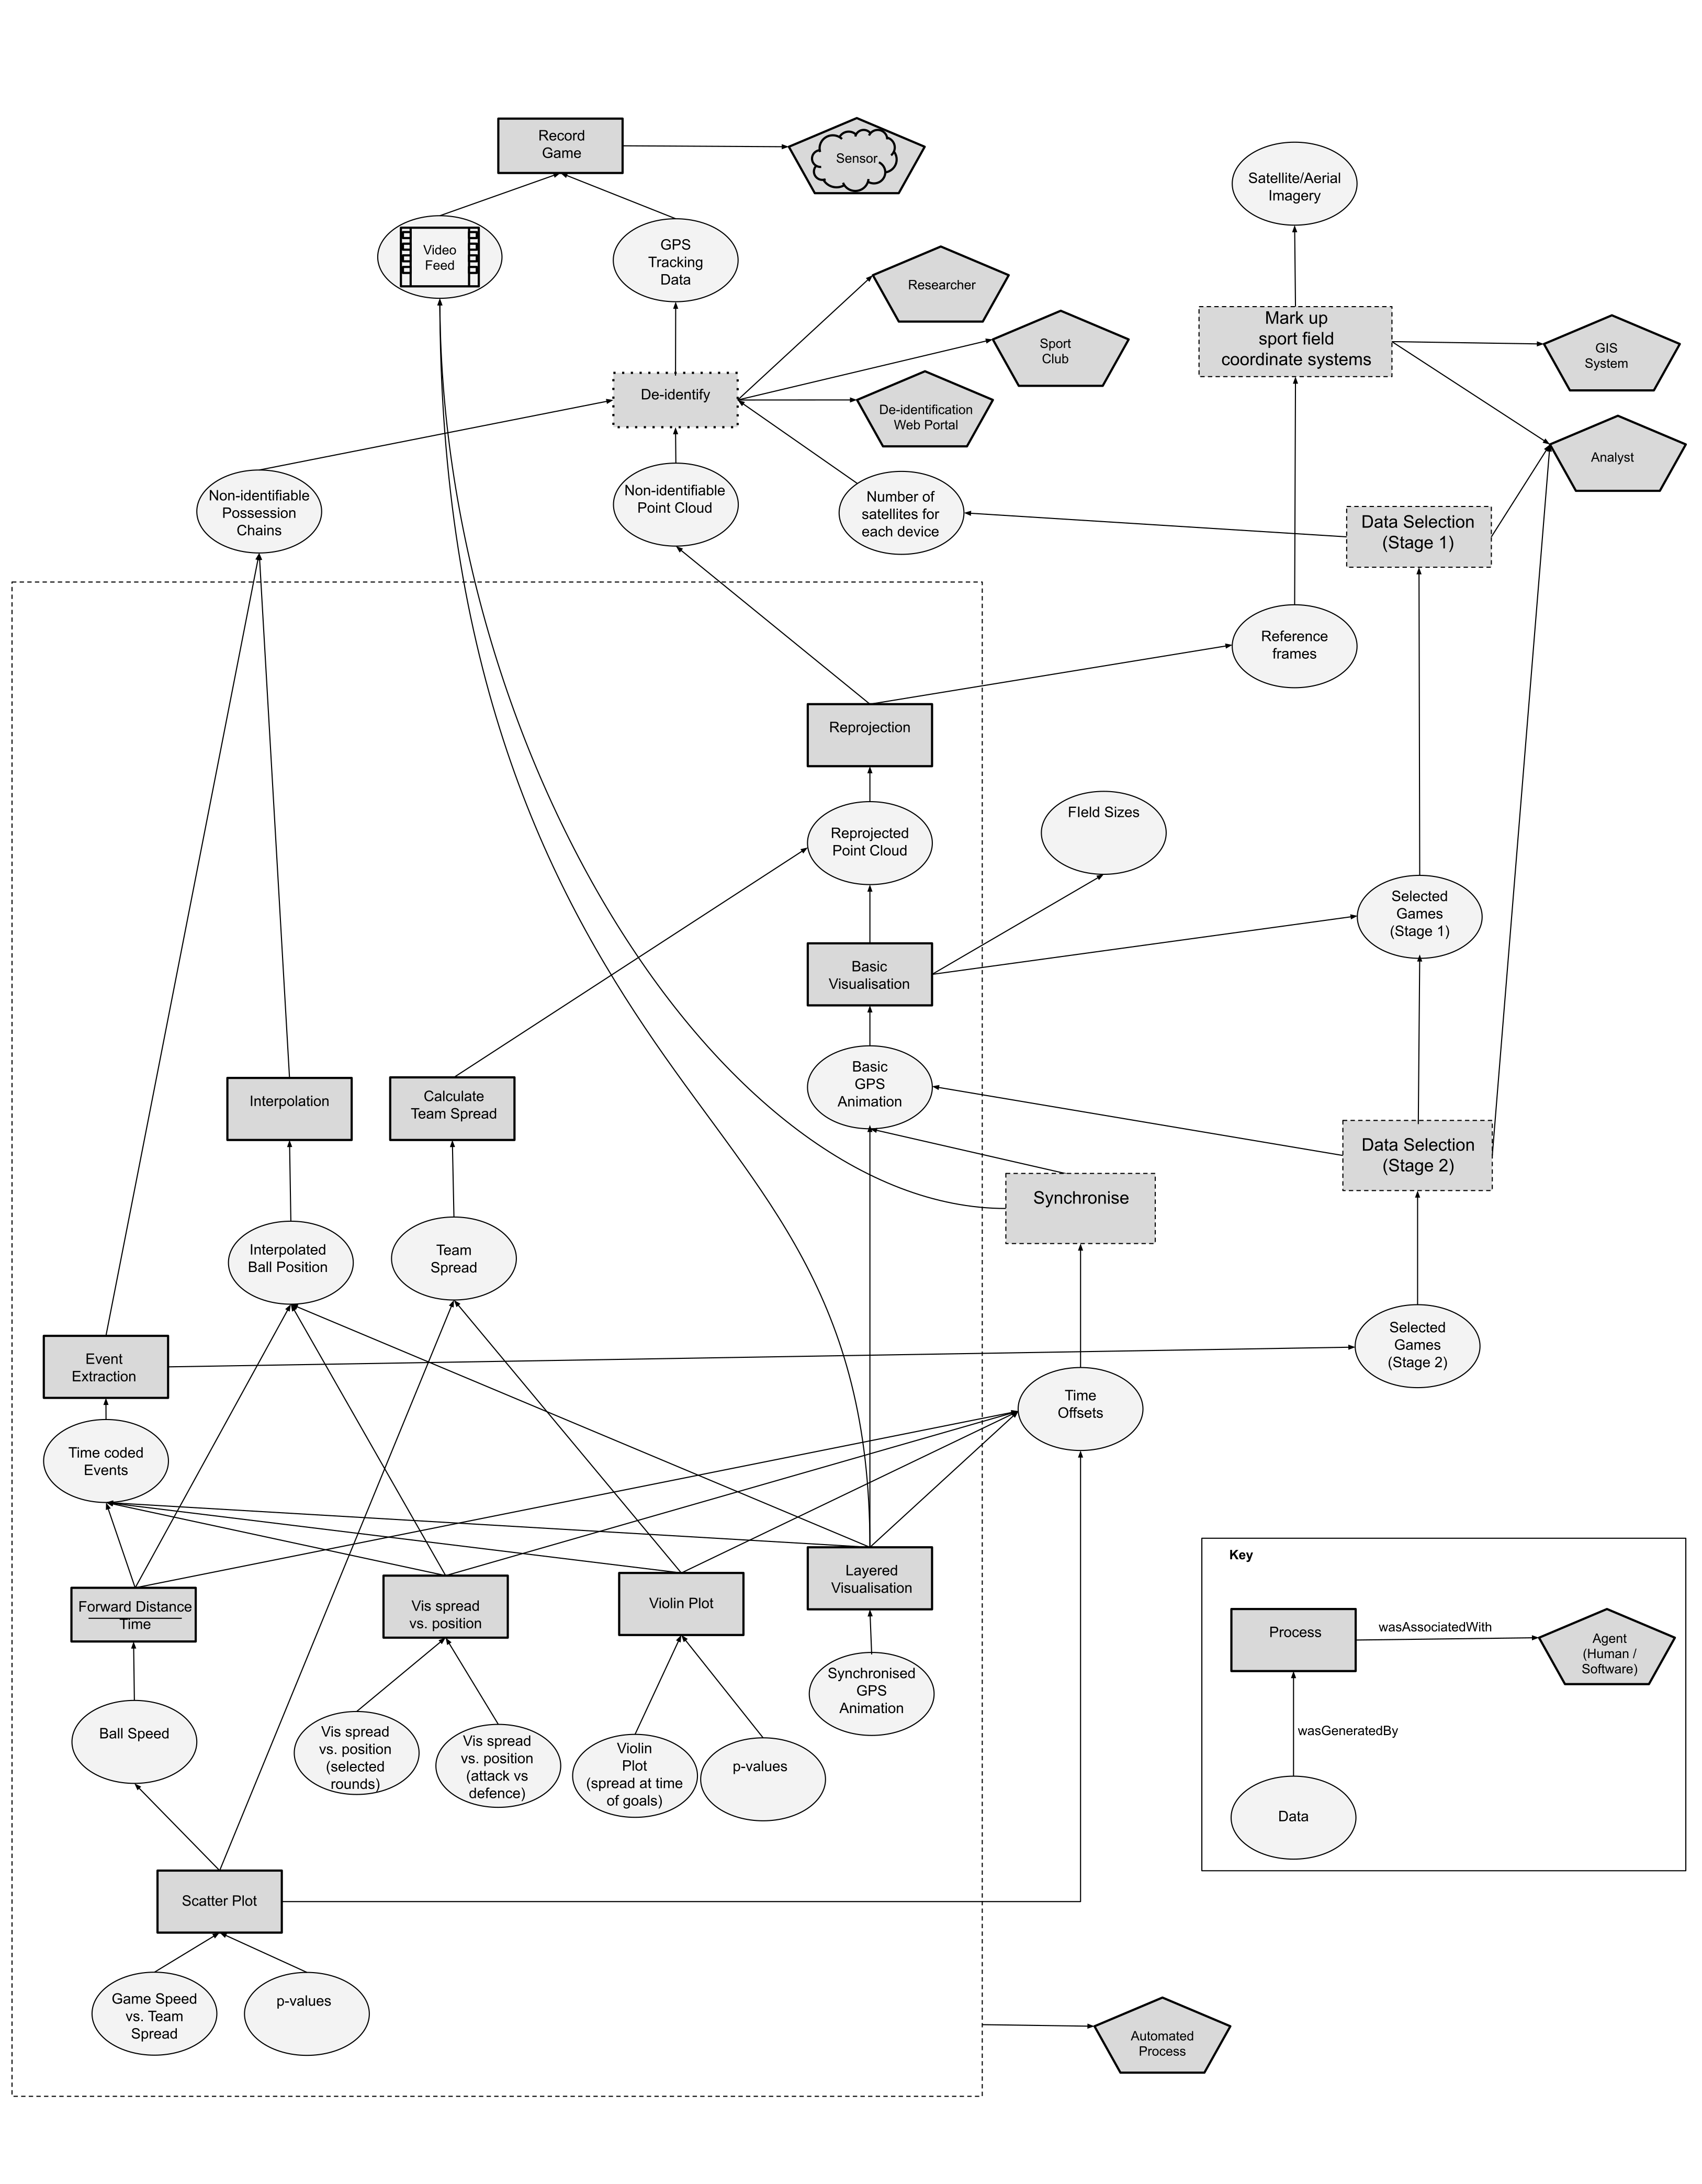
\includegraphics[width=\linewidth]{figs/digital-prov-thesis.png}
% \caption{Provenance graph for spatio-temporal analysis of AFL conducted in this chapter
% \label{fig:digital-prov-thesis}}
% \end{figure}

%\newpage{}

\subsection{Possession Chain Data}

Possession chain data for Geelong Football Club's\footnote{Geelong Football Club is an elite \afl{} club. Note that while the name of the club is identified here (as it would not be practical to suppress it), none of the individual player data (beyond public video footage) are identifiable, even to myself.} matches played during the 2015 season\footnote{For details of the number of matches collected before and after filtering see \secref{sec:integration-data-selection-process}.}, in the format collected by Champion Data (the official supplier to the AFL for all competition data), were obtained via the club. 

Based on the findings of Chapter~\ref{ch:de-identification}, the club was requested to completely remove the player name column (as opposed to substituting names with anonymised player codes) prior to providing the data, as this was the most secure means to prevent re-identification attacks against possession chain data outlined in \secref{sec:de-identification-methods-possession-chain}.

This section of the pipeline is illustrated in \figref{fig:prov1b}.

\begin{figure}[hb]
\centering
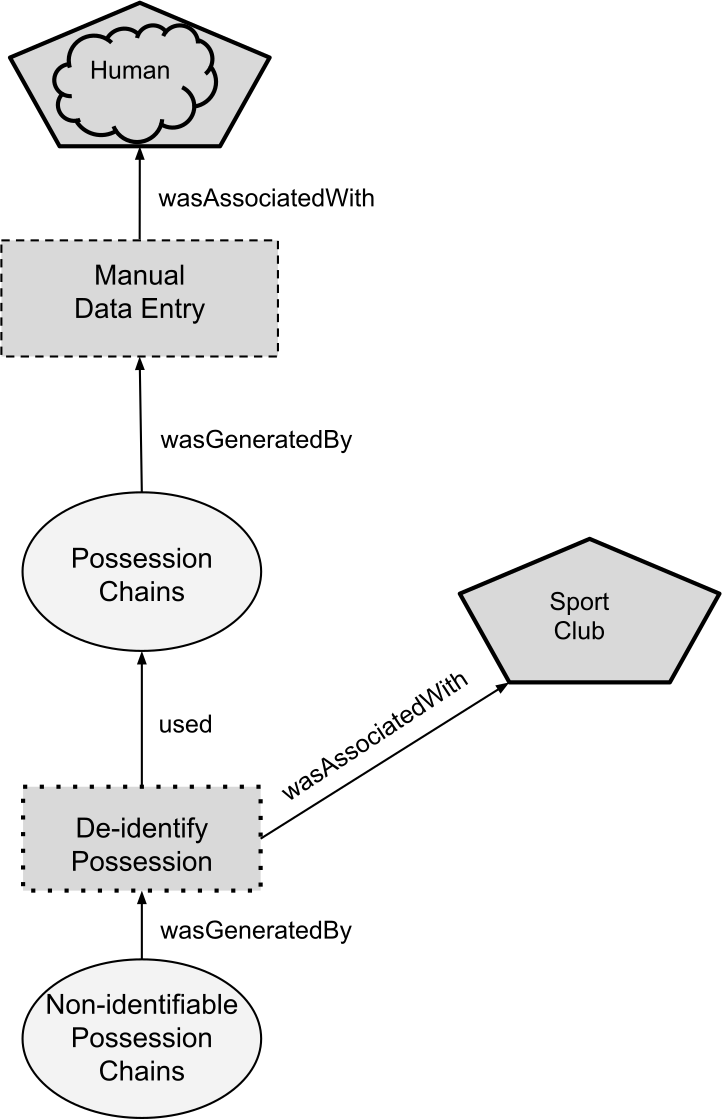
\includegraphics[width=0.6\linewidth]{figs/prov/prov-1-b.png}
\caption{Provenance of non-identifiable possession chain data used in this thesis \notationdetails{}
\label{fig:prov1b}}
\end{figure}

\subsection{Video Data}

\begin{figure}[H]
\centering
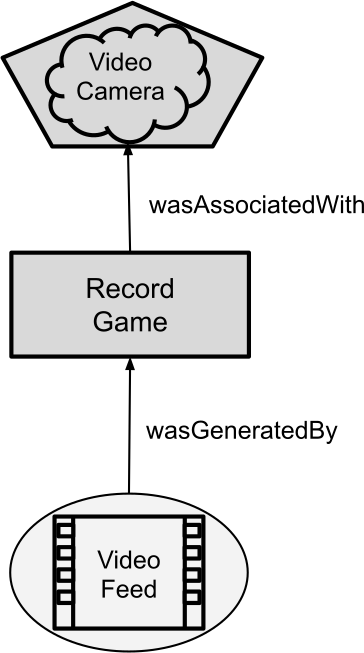
\includegraphics[width=0.3\linewidth]{figs/prov/prov-1-a.png}
\caption{Provenance of video data used in this thesis \notationdetails{}
\label{fig:prov1a}}
\end{figure}

% https://id.afl.com.au/livepass
% https://crowdsupport.telstra.com.au/t5/AFL-Live/AFL-live-pass-match-replay/td-p/734133
% http://www.afl.com.au/livepass/match-replays

% https://www.championdata.com/index.php/sport/afl.html
% "We are the leading and official supplier to the AFL for all competition data"

Televised video recordings of each relevant match were downloaded from the official AFL subscription service (AFL Live Pass match replay) and converted to the MP4 video format for further analysis. The distinction between the digitised video used in this thesis and the original act of recording the game (performed by the broadcaster) is shown in \figref{fig:prov1a}.

Clubs also have access to detailed behind the goals footage, which could be replaced with the televised video recordings used in this thesis if desired. However, as behind the goals footage is neither public\footnote{Clubs are provided with ``exclusive behind the goals vision'' recordings \url{https://www.foxsports.com.au/afl/geelong-coach-chris-scott-explains-why-afl-coaches-bother-going-to-games-inperson-in-2016-with-video-technology/news-story/c9b99fbf9472483491294056c03bf25b}, which are considered a ``game-changer'' for football analysis \url{http://www.afl.com.au/news/2018-02-18/secret-spies-the-life-of-an-opposition-analyst}. A news report in 2013 revealed that clubs payed \$28,000/year each for the footage, with prices expected to rise to \$60,000/year per club in 2014. \url{https://www.theage.com.au/sport/afl/afl-doubles-tv-costs-20131025-2w7d1.html}}, nor non-identifiable\footnote{Even if the club had the resources to blur out faces and player numbers in the behind~the~goals video, the position and movements of players evident within the video would still allow re-identifying particular players in the footage.}, this thesis used the televised video recordings to demonstrate what is possible using only public and/or non-identifiable data.

% https://www.arnnet.com.au/article/570567/technology-could-replace-on-ground-camera-operators-fox-sports/ (seems that broadcasters install their own cameras)
% https://www.theage.com.au/sport/afl/afl-eyes-goalline-cameras-20140226-33iil.html "Television broadcasters"

% \footnote{As the AFL does not officially offer a download option, M3U8 playlists describing the transport stream for each match quarter were extracted from the HTML video playback interface. The video segments referenced in each stream were fetched from the Telstra CDN using \texttt{wget}, and then concatenated to reconstruct the video file for each quarter. \url{https://stackoverflow.com/questions/22188332/download-ts-files-from-video-stream/32044464\#32044464}}

%\newpage{}

\subsection{GPS Data}
\label{sec:gps-data-selection}

\begin{figure}[H]
\centering
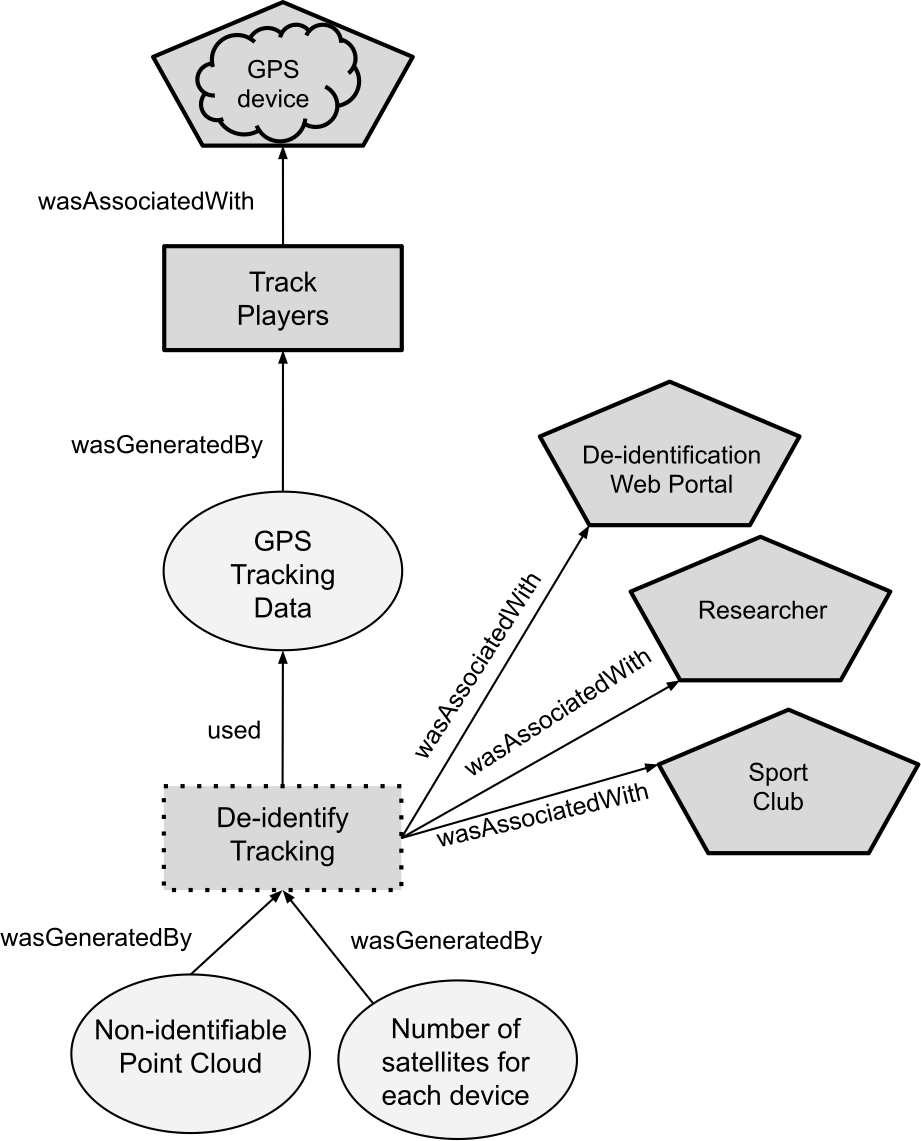
\includegraphics[width=0.7\linewidth]{figs/prov/prov-1-c.png}
\caption{Provenance of non-identifiable point cloud data used in this thesis \notationdetails{}
\label{fig:prov1c}}
\end{figure}

Player GPS tracking data were requested, where available, for Geelong Football Club's 2015 matches. The data were requested and anonymised using the \textit{deidentify.org} portal \cite{Simmons2018} designed as part of this thesis for the purpose of addressing the issues described in Chapter \ref{ch:de-identification}. This section of the pipeline is illustrated in \figref{fig:prov1c}. The data extraction requests are listed in \appendixsecref{appendixsec:data-extraction-request}.

\subsection{Data Selection Process}
\label{sec:integration-data-selection-process}

\begin{figure}[H]
\centering
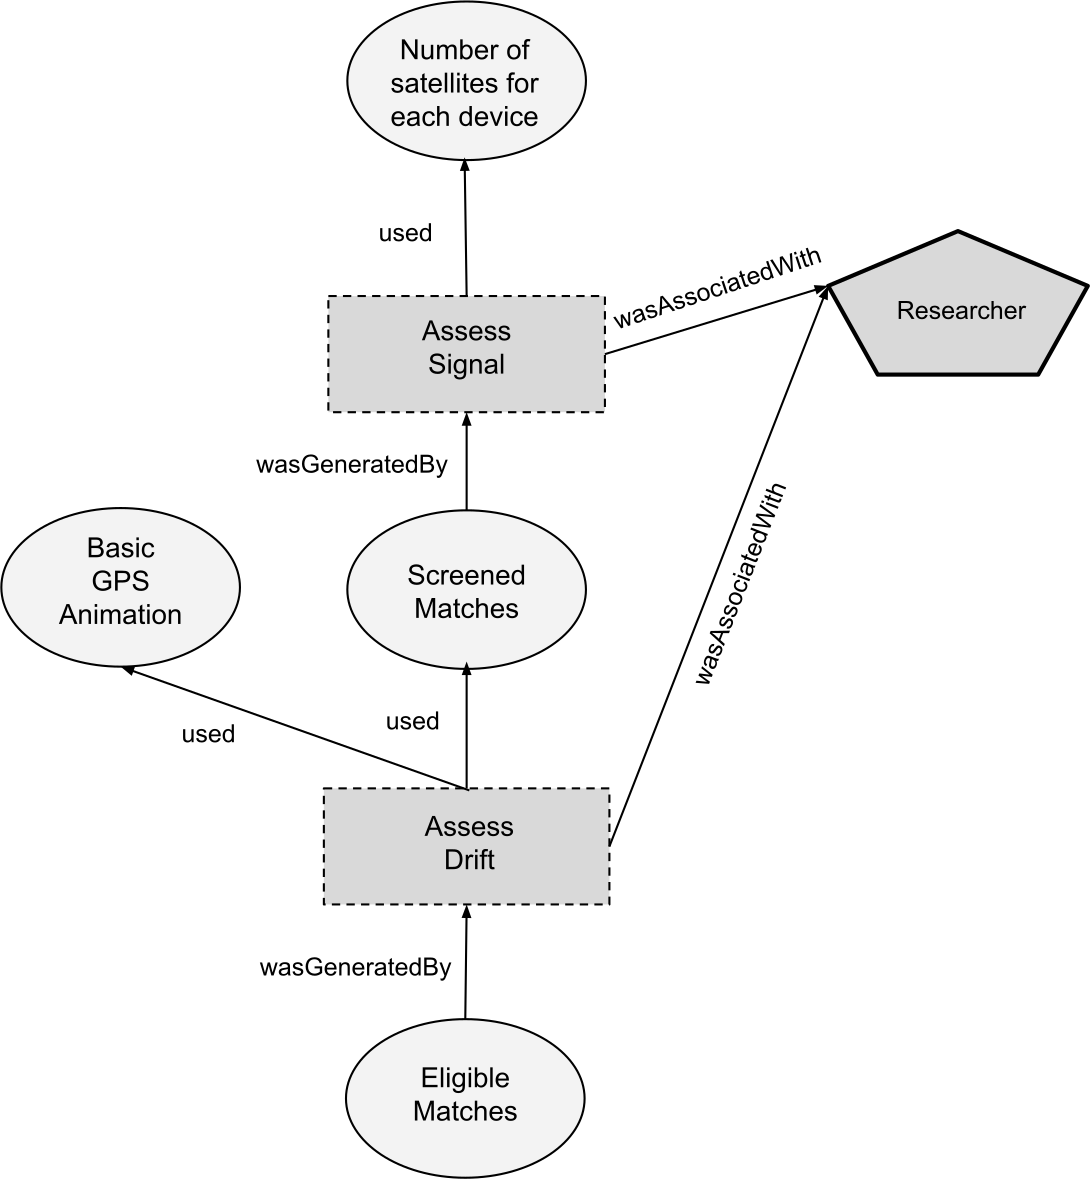
\includegraphics[width=0.8\linewidth]{figs/prov/prov-2.png}
\caption{Provenance of eligible \afl{} match list used in this thesis \notationdetails{}. The Basic GPS Animation used for visual inspection of potential data issues is described in \secref{sec:integration-vis}.
\label{fig:prov2}}
\end{figure}

\begin{figure}[htbp]
\centering
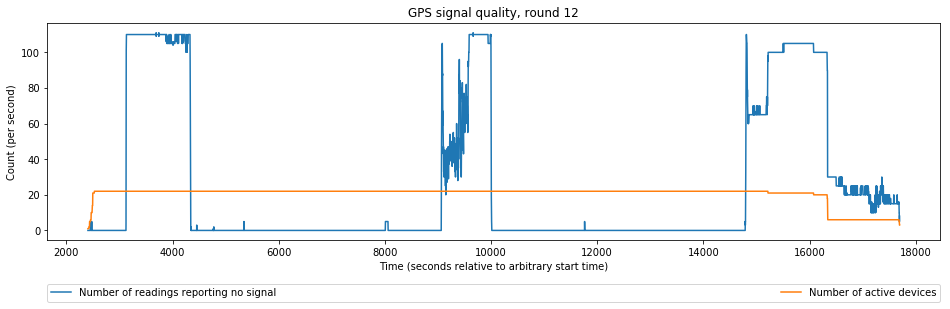
\includegraphics[width=\linewidth]{figs/model/geelong_gps_qual_r12.png}
\caption{GPS signal quality inspection for round 12. All 22 devices (orange) were active during the match. The (blue) peaks in devices reporting no signal are the moments that the team is off field, prior to the game, during the mid-game break, and after the game. As the GPS data provided by the club was exported at a sample rate of 5~Hz, the number of readings reporting no signal per second can reach approximately 5 times that of the number of active devices. While the plot shows there were some instances of signal loss while the game was in play, these are negligible compared to the proportion of the game that had clear signal, and hence this match was included in the analysis.}
\label{fig:gps-qual-example}
\end{figure}

% PRISMA flow diagram (aka study attrition diagram) image
\begin{figure}[!htb]
  \centering
  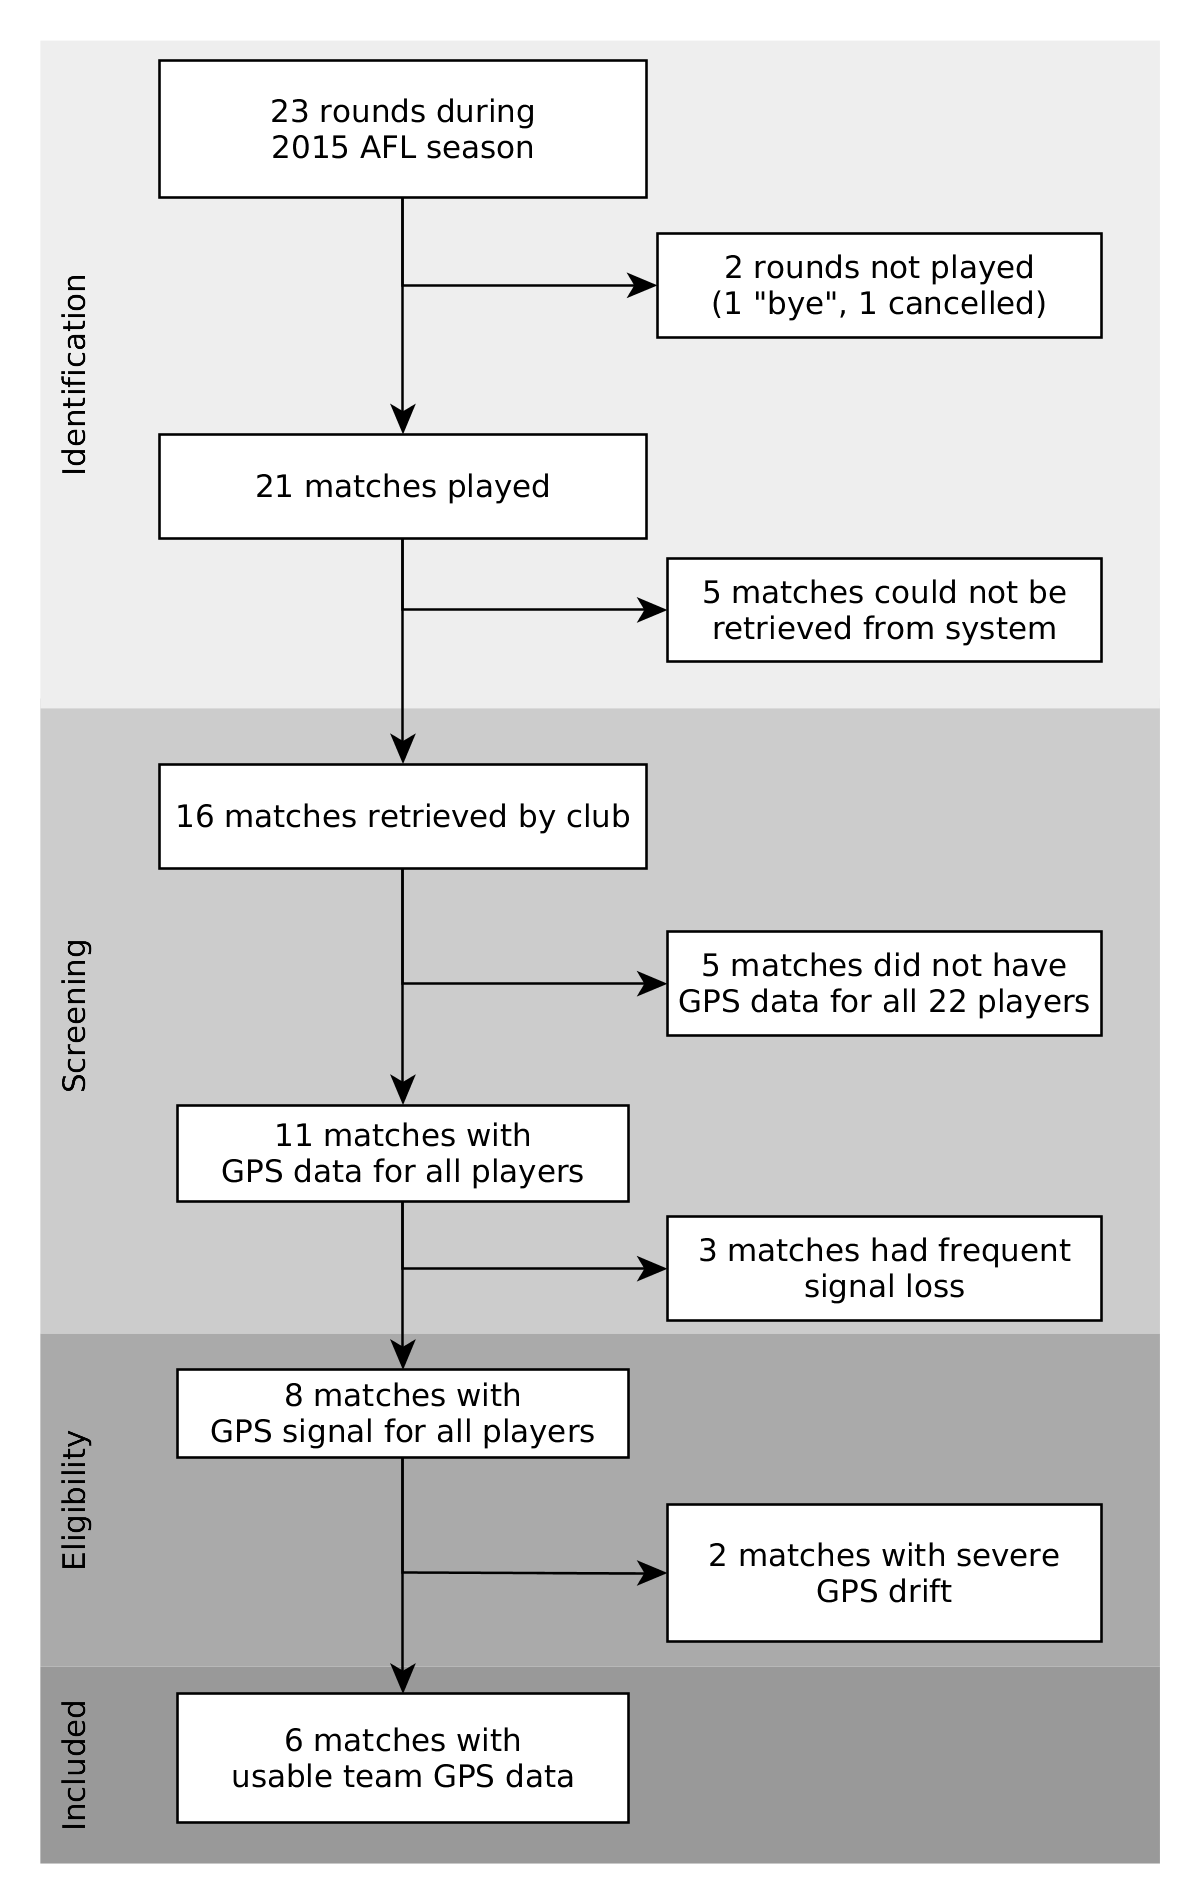
\includegraphics[width=0.8\linewidth]{round-selection}
  \caption{Match selection}
  \label{fig:prisma-round-selection}
\end{figure}

\figref{fig:prov2} provides an overview of how the GPS data for each match were screened and assessed for data quality. Geelong Football Club played 21 out of 23 rounds in 2015 (round 13 was a ``bye'' round for the club in which they were not scheduled to play, and
round 14 was cancelled after the death of an \afl{} coach).
Of the 21 matches played during 2015, the performance team at Geelong Football Club were able to retrieve GPS data for 16 matches. It was necessary to exclude five of the retrieved matches from the analysis because they did not contain data for all 22 players. A further three rounds were excluded due to frequent signal loss over the course of the entire duration of the game. This left eight matches that had periods of whole-team GPS data during the game. Upon closer inspection, it became apparent that in two of the matches, the GPS devices were active, but there was severe interference near the interchange area causing players who were off field near the interchange area to be reported as if they were at mid-field. While this could have been corrected with identifiable data (i.e. knowledge of which players were benched at which times) to exclude the trace, the non-identifiable point cloud representation made it impossible to distinguish spurious locations in which benched players were reported as being on the field from cases where players were actually on the field. As such, these two rounds were also excluded from the analysis. This left a total of six matches with good data (five of which were played at the team's home ground).

An example of signal quality for one of the selected rounds is provided in \figref{fig:gps-qual-example}. \figref{fig:prisma-round-selection} shows the number of matches that needed to be discarded at each stage of the selection process due to GPS data issues.


% \todo{Check this information (not all GMHBA, UNSW not coded, MCG round 1 coded but shouldn't have been) (count seems to be incorrect!)}
% Checked and updated. 6 good games (5 games at home ground, 1 at UNSW)

\subsection{Reprojection} \label{sec:integration-reprojection}

\begin{figure}[H]
\centering
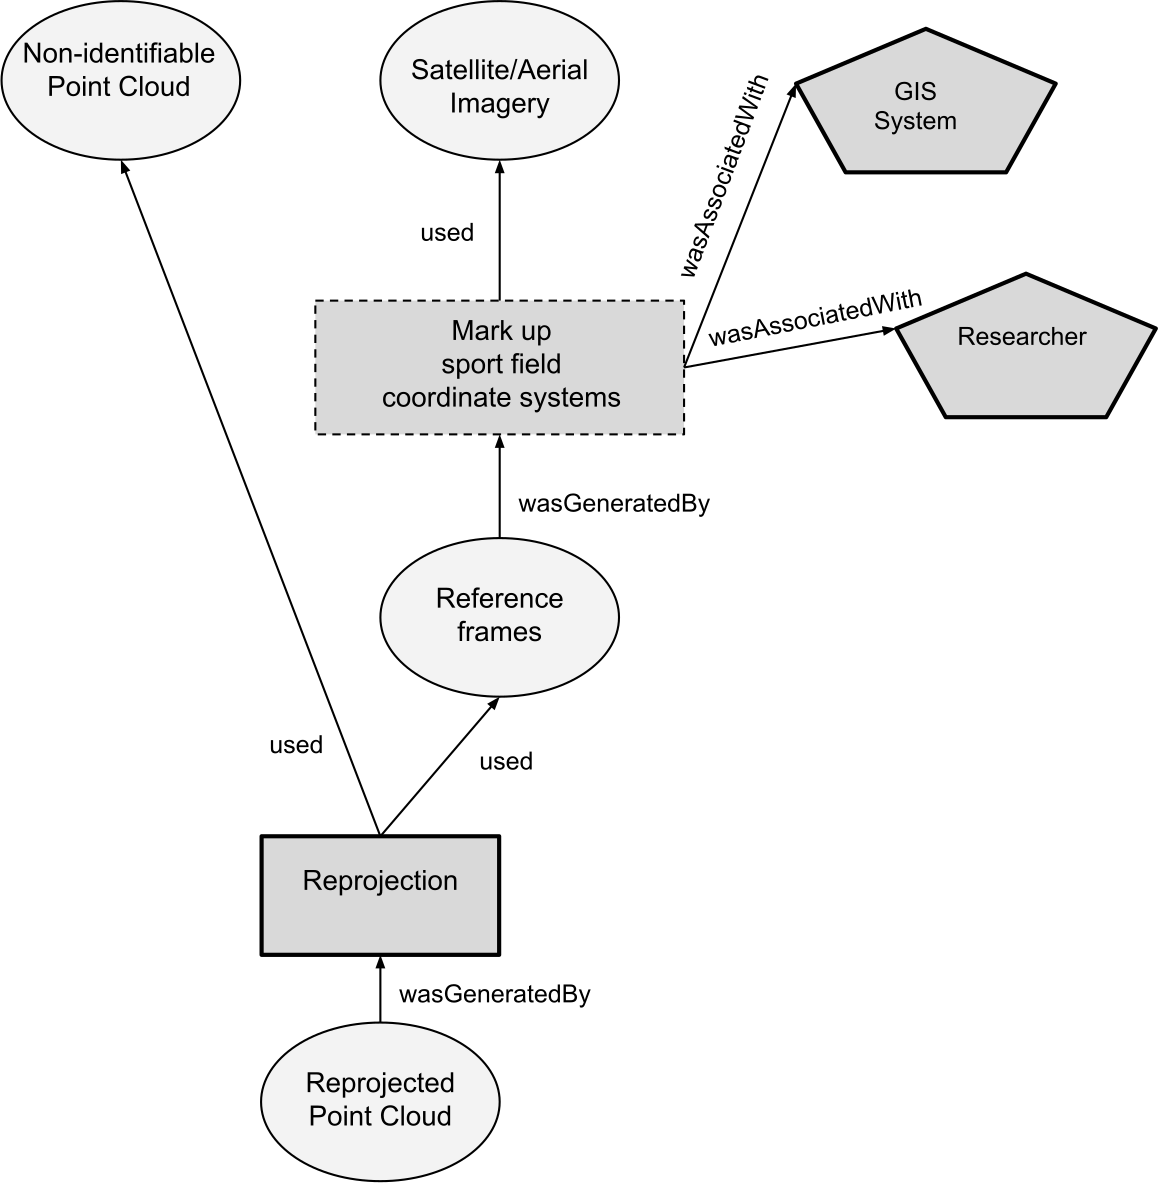
\includegraphics[width=0.9\linewidth]{figs/prov/prov-3.png}
\caption{Provenance of reprojected point cloud used for visualisation and analysis \notationdetails{}
\label{fig:prov3}}
\end{figure}

\begin{figure}[htbp]
\centering
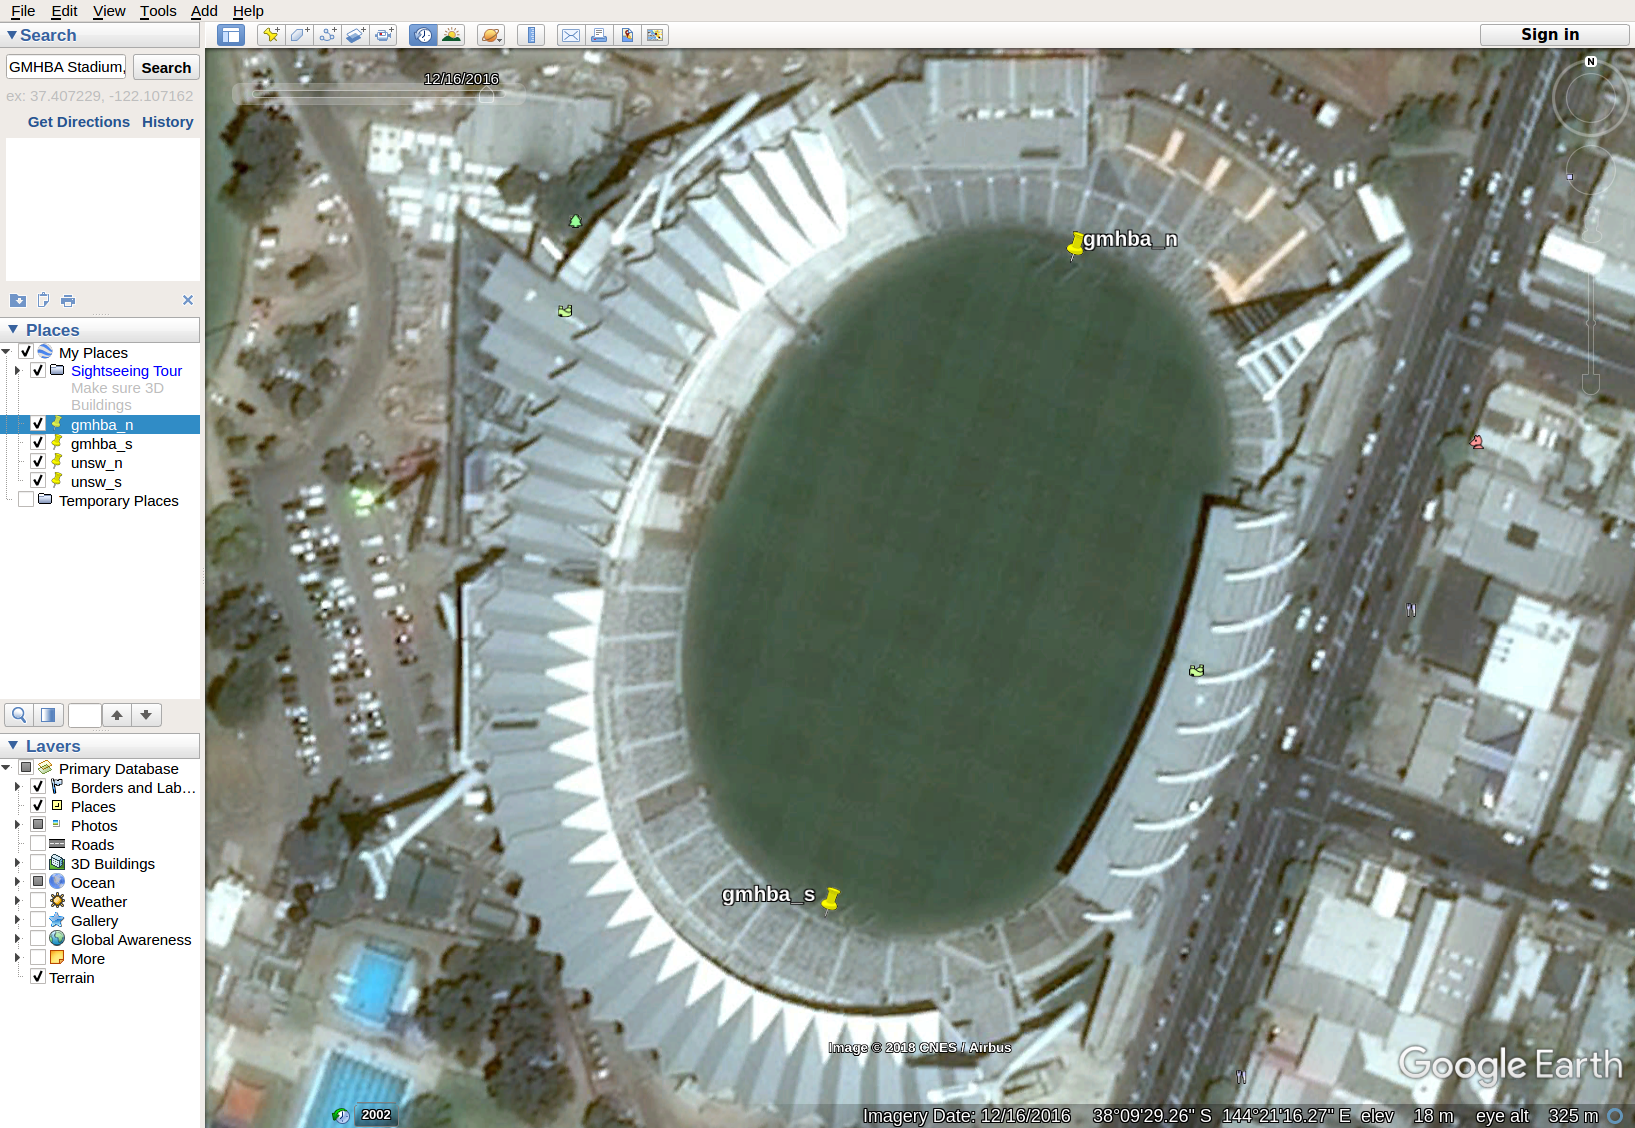
\includegraphics[width=0.8\linewidth]{goog-earth-gmhba.png}
\caption{Historic satellite and aerial imagery available through Google Earth Pro was used to estimate the coordinates of the goals (yellow pins) at each stadium.}
\label{fig:gps-pinpoint-example}
\end{figure}

\figref{fig:prov3} shows the pipeline to pipeline to reproject the player GPS tracking data relative to the field. The first task towards marking up the sport field coordinate system was to determine the location of the goal posts. The goal posts were located using Google Earth Pro, as it included high resolution satellite and aerial imagery of each field, as well as the ability to look at past imagery during the 2015 season to confirm that the shape of the oval had not changed (e.g. due to resurfacing the oval). An example of pinpointing the goals of Kardinia Park (commercially known as GMHBA stadium) is shown in \figref{fig:gps-pinpoint-example}.

\newpage{}

Once the location of the goal posts were determined, these were converted to a geographic file (in the GeoJSON format) specifying a line from the goal area at one end of the field to the goal area at the opposite end of the field, for each venue. These were used to establish reference frames for each venue, as per the \textit{Spatio-Temporal Reference Frames As Geographic Objects} method \cite{Simmons2017} proposed in Chapter~\ref{ch:spat-trans}. As the time attribute in the GPS data provided by the \afl{} club contained minutes and seconds but was stripped of the date and hour part, it was not possible to automatically determine which venue GPS data corresponded to based on the time period alone. As such, a special ``\texttt{filt\_radius}'' property was added to venues to inform the processor to use that venue as the reference frame whenever the GPS data fell within that radius of the venue. An example of the GeoJSON input to the processor is provided in Listing~\ref{lst:geojson}.

Once reference frames are established, the processor also requires a directory of GPS data to reproject, which was the de-identified GPS point clouds obtained from the club (\secref{sec:gps-data-selection}).

\newpage{}

\begin{lstlisting}[
  language={},
  numbers=none,
  label=lst:geojson,
  caption={Contents of \texttt{venue\_refs.geojson}. The location and orientation of each venue is recorded via a LineString drawn between the two ends of the field. As the GPS data provided by the club did not contain the date or hour part, the time is kept as is (\texttt{"abstime"}) and synchronised with match footage later in the process. A radius (\texttt{filt\_radius} = 500 metres) is specified for each venue and used to automatically reproject any GPS data falling within that proximity to the coordinate system of the venue},
  basicstyle=\ttfamily
]
{
  "type": "FeatureCollection",
  "crs": {
    "type": "name",
    "properties": {
       "name": "urn:ogc:def:crs:OGC:1.3:CRS84"
     }
  },
  "features": [
    {
      "type": "Feature",
      "properties": {
         "GMHBA": "abstime",
         "filt_radius": 500
       },
       "geometry": {
         "type": "LineString",
         "coordinates": [
           [144.354250252864091, -38.158864651758321],
           [144.354946985064288, -38.157403511709113]
         ]
       }
    },
    ...
  ]
}
\end{lstlisting}

\subsection{Visualisation} \label{sec:integration-vis}

\begin{figure}[H]
\centering
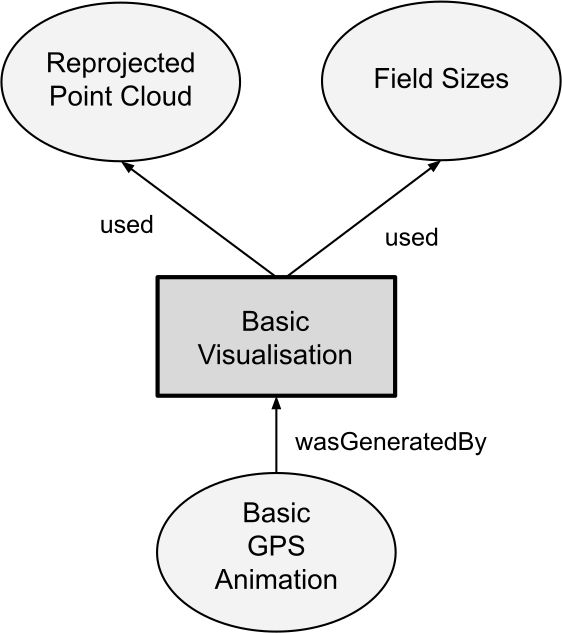
\includegraphics[width=0.45\linewidth]{figs/prov/prov-4.png}
\caption{Provenance of basic GPS animation developed for this thesis \notationdetails{}
\label{fig:prov4}}
\end{figure}

\begin{figure}[htbp]
\centering
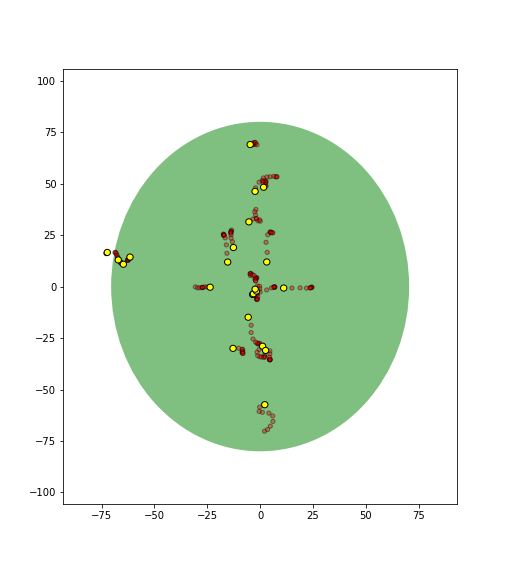
\includegraphics[width=0.3\linewidth]{gps_frames_selected_r22/frame2650.png}
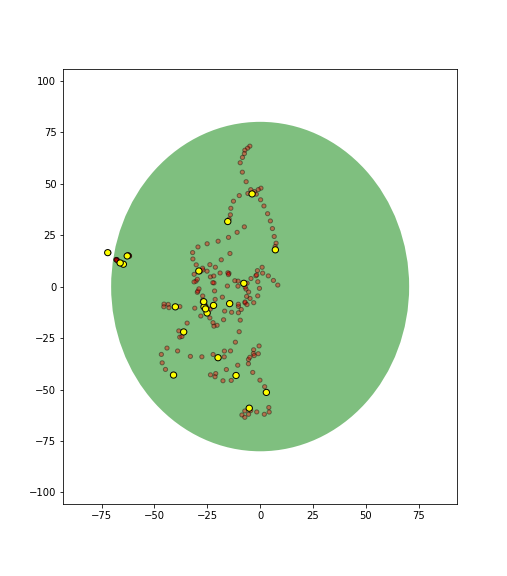
\includegraphics[width=0.3\linewidth]{gps_frames_selected_r22/frame2660.png}
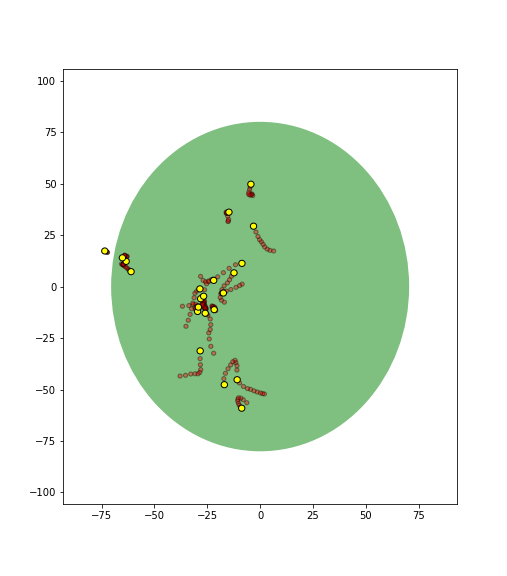
\includegraphics[width=0.3\linewidth]{gps_frames_selected_r22/frame2670.png}
\caption{Visualisation of player positions for a play during the 2015 grand final. Left: \centrebounce{} formation. Middle: 10 seconds after \centrebounce{}. Right: 20 seconds after \centrebounce{}. Yellow dots indicate position of players, and red trails indicate past positions (logged at 1 Hz). The distance between each consecutive red dot in the trail is distance moved each second, and is thus an indication of player speed.}
\label{fig:gps-frames-selected}
\end{figure}

The reprojected GPS data were then visualised and overlaid on a background indicating the field shape (see \figref{fig:prov4}). An example of this visualisation for various moments during a game is shown in \figref{fig:gps-frames-selected}. To give an indication of the movement and speed of the players, the visualisation includes a trail of previous player positions. Note that as a non-identifiable point cloud representation was used, there is no internal representation of which past time points belong to which player; however, the visualisation shows that the path of players over time can still be visually tracked for short periods other than at moments when players come within close proximity to another player. By design, it is ambiguous which player belongs to which trail beyond the point where players cross paths with each other.

\subsection{Time Synchronisation}
\label{sec:integration-timesync}

\begin{figure}[H]
\centering
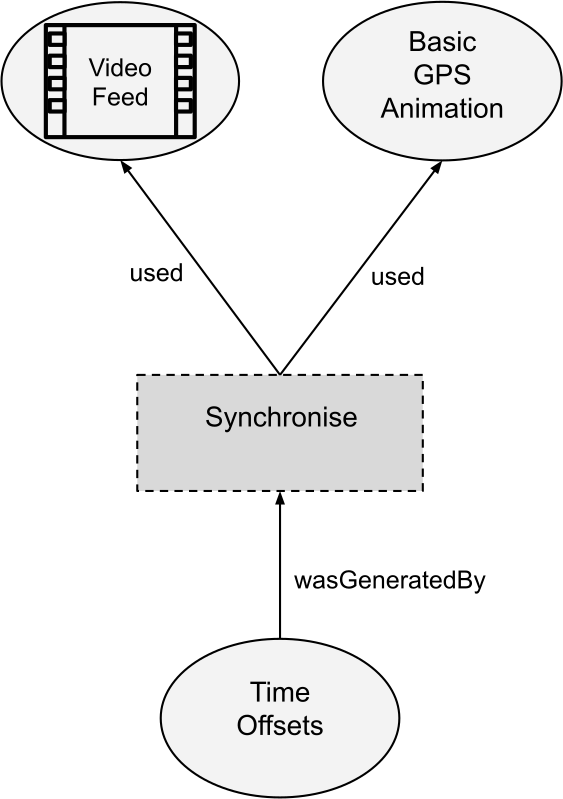
\includegraphics[width=0.45\linewidth]{figs/prov/prov-5.png}
\caption{Provenance of time offsets used in this thesis \notationdetails{}
\label{fig:prov5}}
\end{figure}

\begin{figure}[htbp]
  \centering
  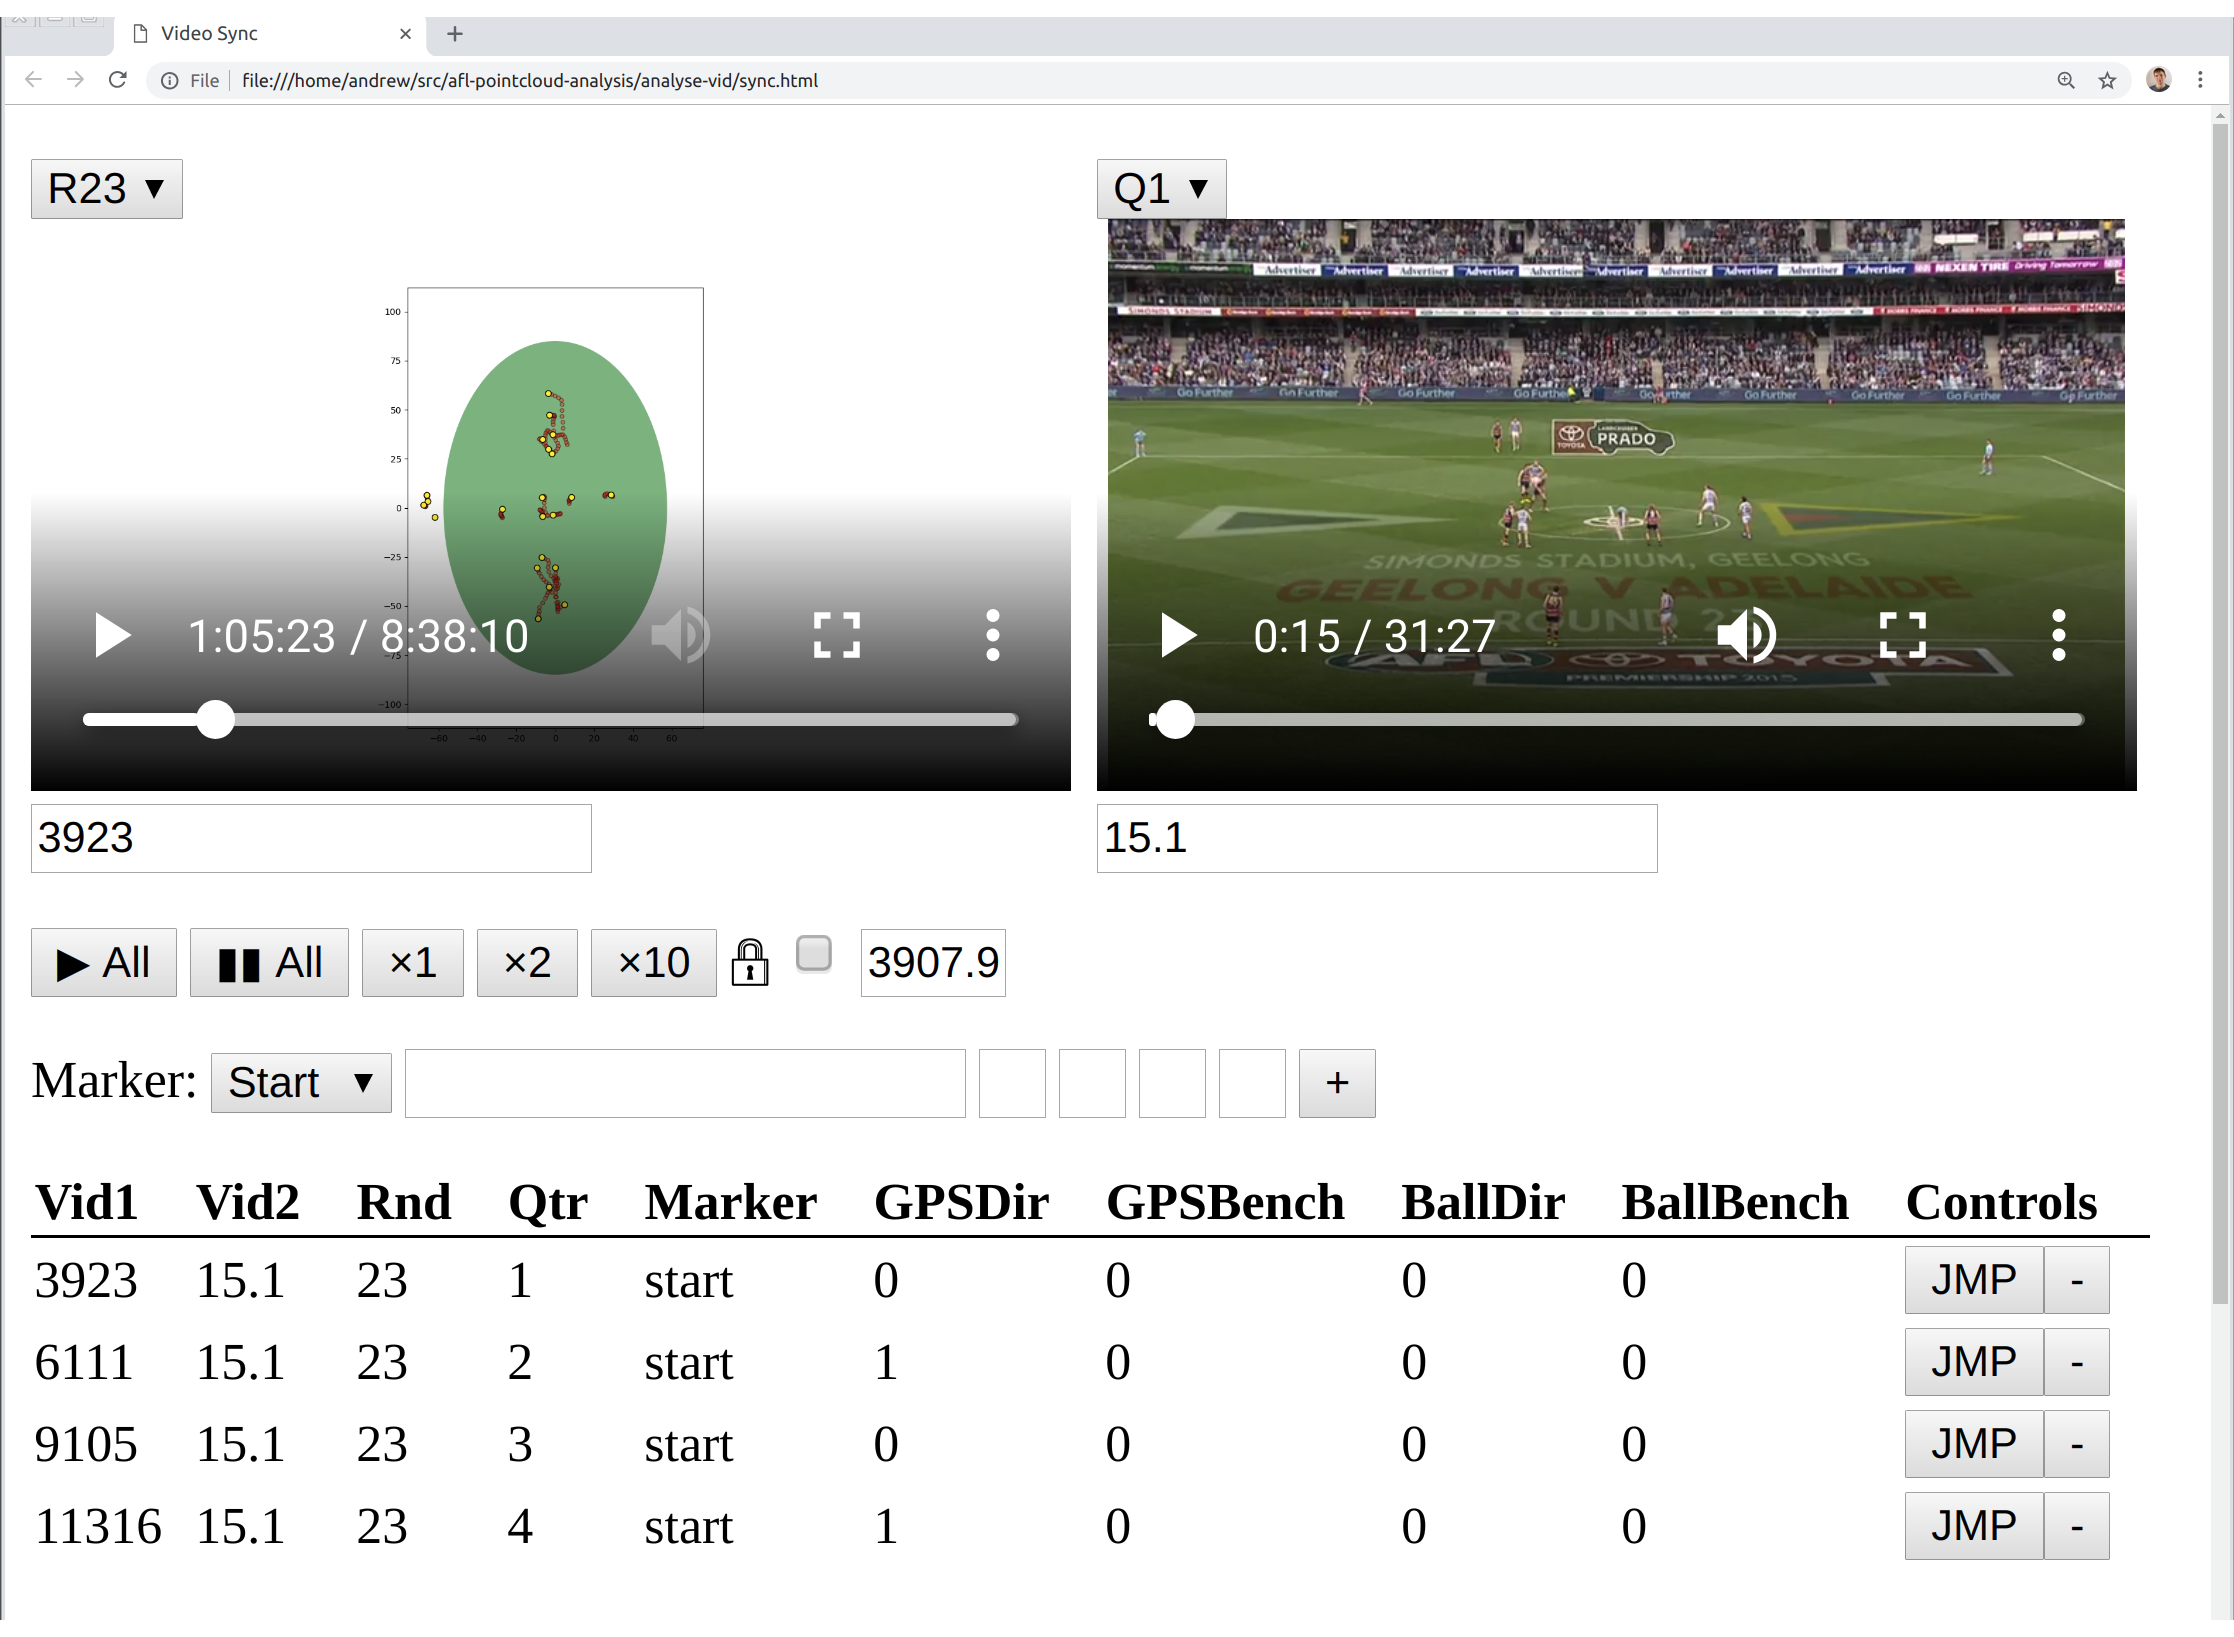
\includegraphics[width=\linewidth]{scrshot-video-sync}
  \caption{Video synchronisation tool}
  \label{fig:scrshot-video-sync}
\end{figure}

The GPS visualisation was turned into an animation, showing the current player formation and a 10 second trail of past movements. The animation was then synchronised with video of the game using a custom tool designed for this thesis (shown in \figref{fig:scrshot-video-sync}) in order to obtain the time offsets (see \figref{fig:prov5}). Any event can be used to synchronise the video and animation; in practice the \centrebounce{} at the start of each match was used, as the sudden change in motion provides a clear indicator of when this event occurs.

A key feature of the tool is that once the user has found the approximate offset between the animation and the video feed, they can lock the offset then scrub through the video to verify that the alignment is correct. For example, in one video the first \centrebounce{} formation in the animation was synchronised with the first \centrebounce{} in the match video, but scrubbing through the video to verify the alignment revealed that moments later in the video didn't align with the GPS animation. Investigating this further revealed that the video recording was started late and opened with the second \centrebounce{} of the game rather than the first. Upon reporting this issue, the official video provider confirmed the error and uploaded the complete match footage.\footnote{[Issue] Andrew Simmons, ``First 30 seconds of Q4 match replay is missing - Geelong vs Melbourne, Round 12, 2015'', Telstra support \url{https://crowdsupport.telstra.com.au/t5/AFL-Live/First-30-seconds-of-Q4-match-replay-is-missing-Geelong-vs/m-p/790084\#M6776}}

\subsection{Synchronised Visualisation}

\begin{figure}[H]
\centering
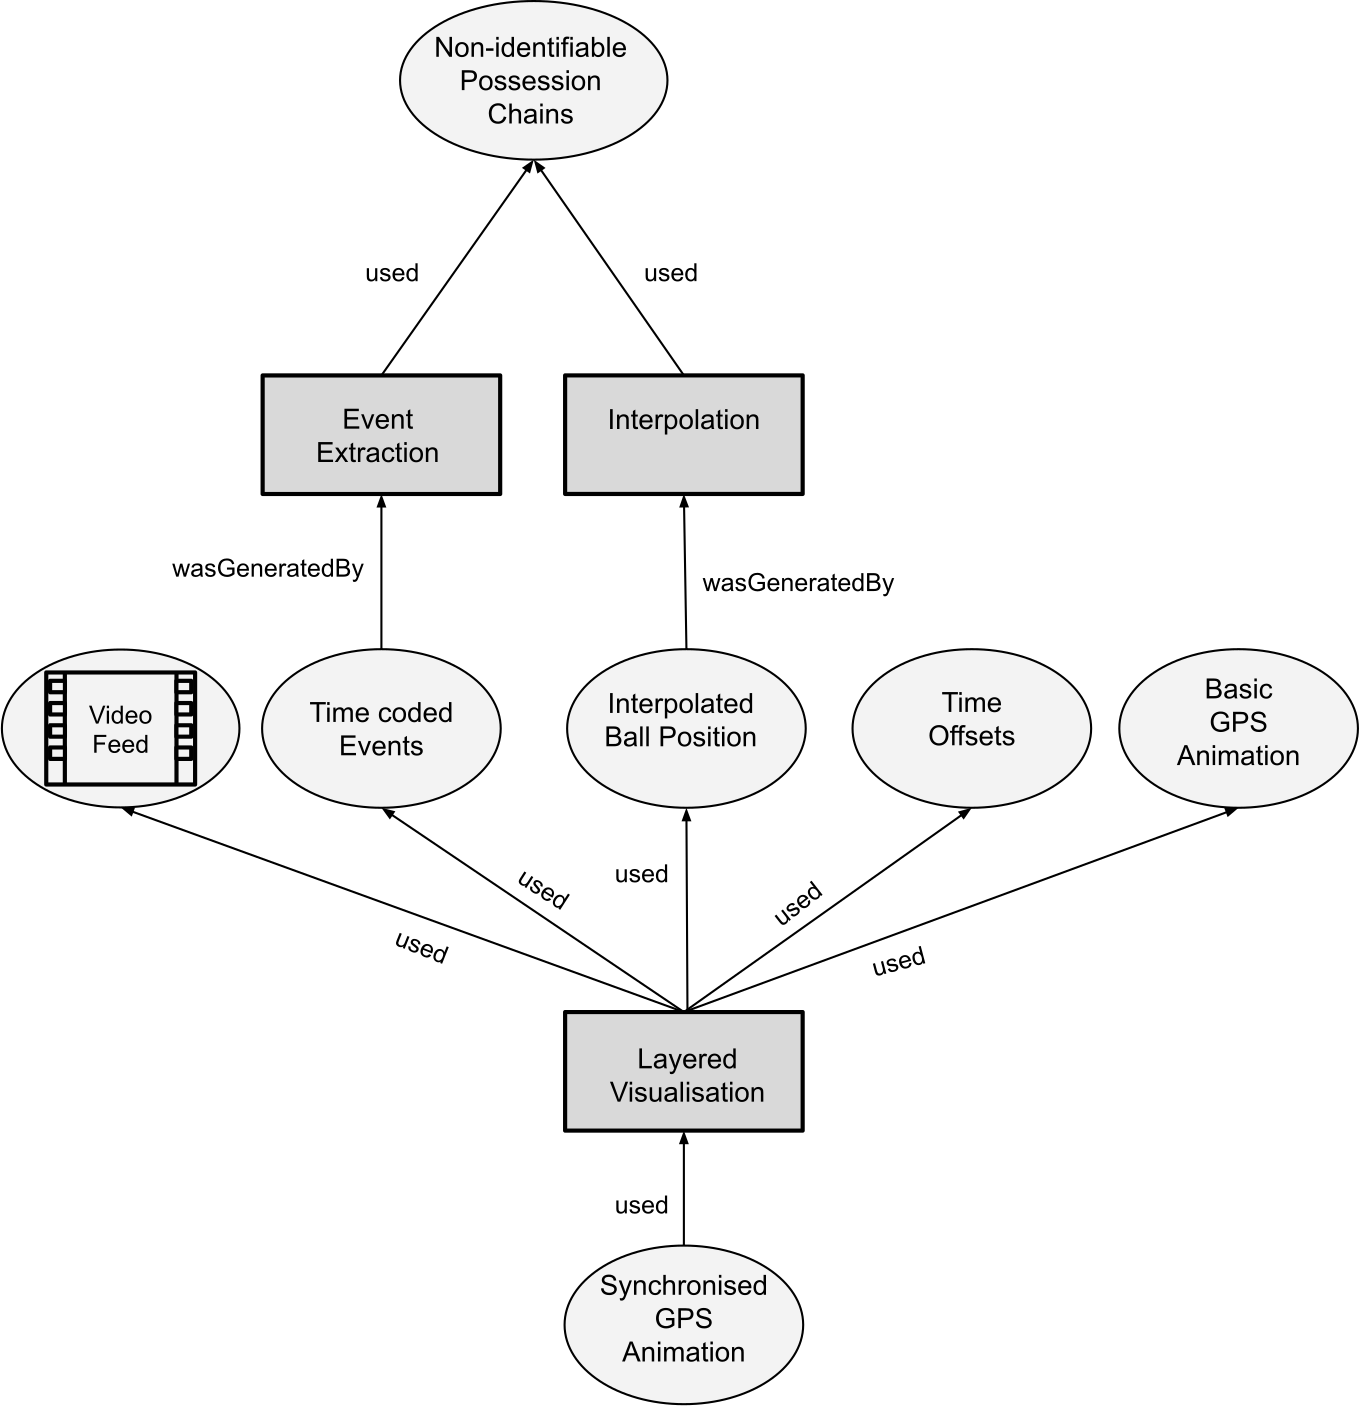
\includegraphics[width=\linewidth]{figs/prov/prov-6.png}
\caption{Provenance of synchronised GPS animation developed for this thesis \notationdetails{}
\label{fig:prov6}}
\end{figure}

\pagebreak{}

Once the GPS data had been synchronised with the video, other data sources were integrated, such as Champion Data possession chains. This section of the pipeline is illustrated in \figref{fig:prov6}.

Note that the possession chain timestamps were expressed relative to the start of each quarter, so this alignment was only possible once the synchronisation of GPS data with match video was complete. Champion Data also record the approximate ball location, which they manually pinpoint at key moments during the game. As there is no GPS tracker in the ball, these approximate ball locations were used to provide an approximate ball location feature. \afl{} clubs use video analysis tools to record their own annotations of the game (e.g. personal communication with the club revealed that they manually annotate the timeline with moments of key player decisions to review). The club did not share these, but if available they could have also been incorporated once the video synchronisation process was complete.

Additionally, during this stage the direction of attacking goals (i.e. which end of the field teams attempt to head towards) was annotated using the tool via manual observation of the animation.\footnote{Teams change sides each quarter, with the initial direction of attacking goals determined by a coin flip at the start of the game. However, there did not appear to be publicly recorded data on coin flips in a form that could be readily translated into a spatial heading.} Due to the tendency of the team to chase after the ball, it is possible that this step could be automatically inferred based on which side of the field the team is on at the moments they score a goal. However, as it is critical to the results of the analysis that the direction of attacking goals was determined correctly, this was annotated manually instead.



\pagebreak{}

\begin{figure}[!htb]
  \centering
  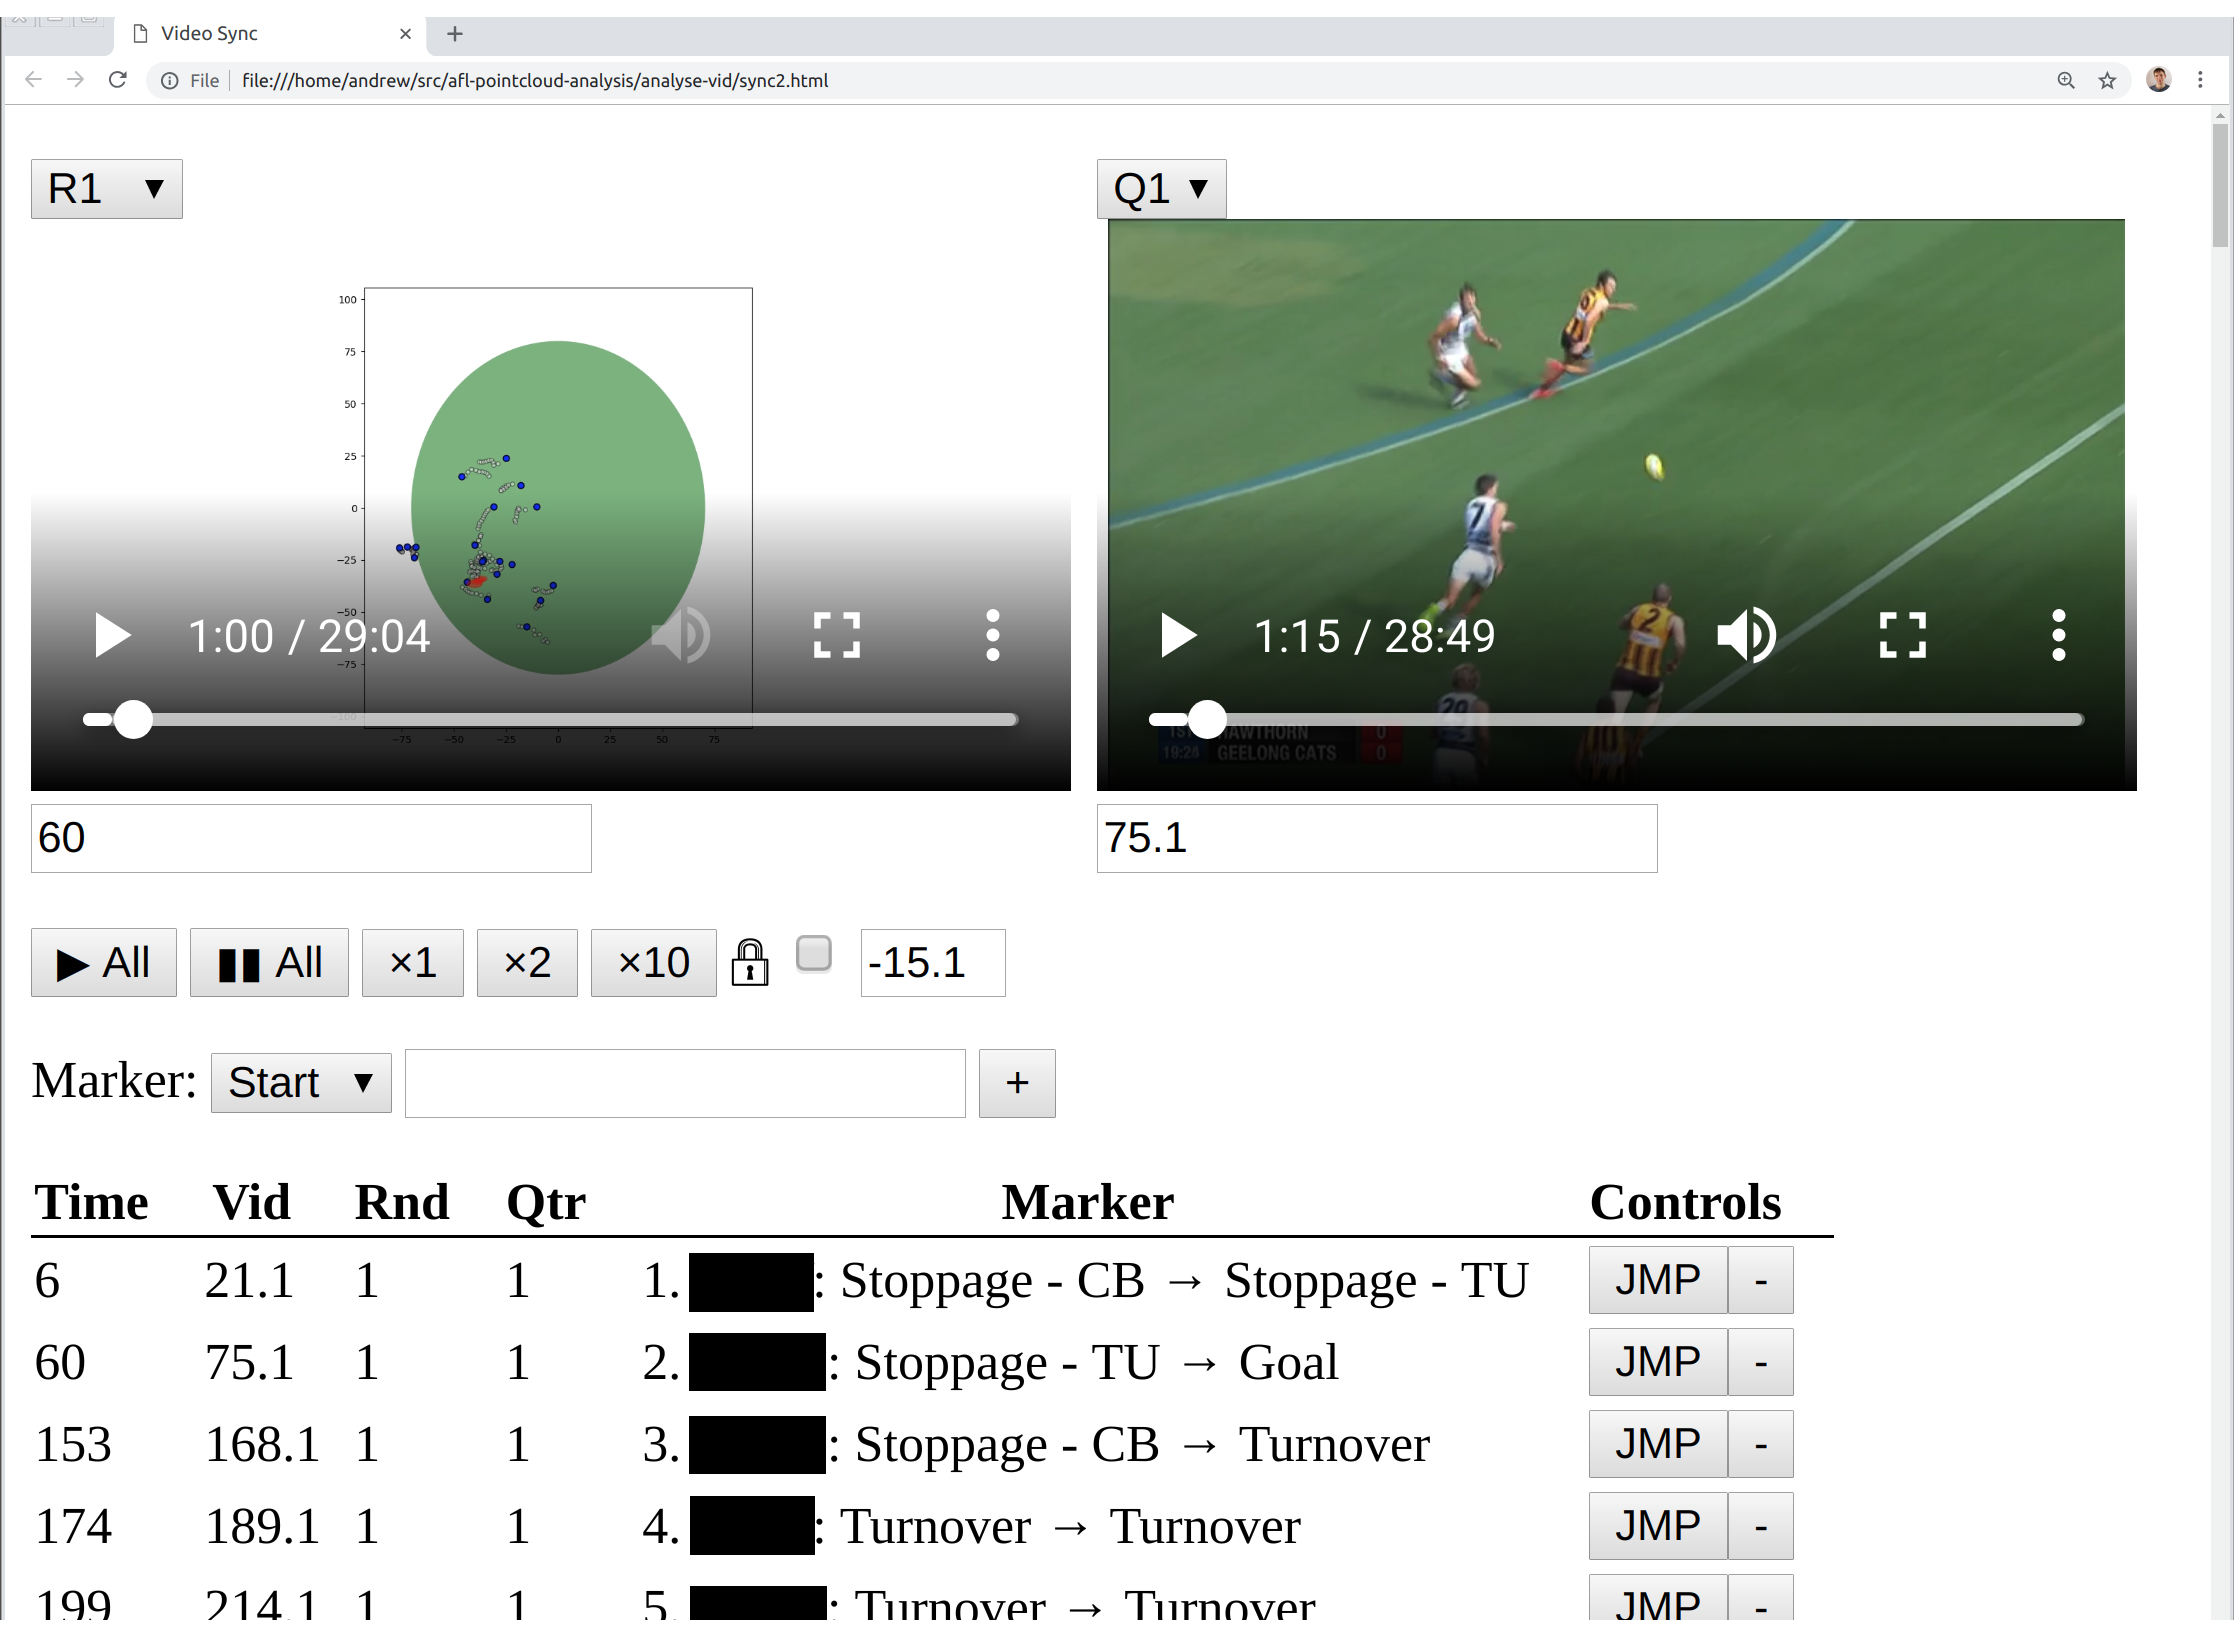
\includegraphics[width=\linewidth]{scrshot-video-sync-layer2}
  \caption{Synchronised visualisation}
  \label{fig:scrshot-video-sync-layer2}
\end{figure}

The synchronised visualisation is shown in \figref{fig:scrshot-video-sync-layer2}. Note the list of key events shown at the bottom of the interface, as imported from Champion Data possession chain data after synchronisation. Similar commercial video analysis tools, such as Sportscode could be used for this (i.e. annotating and exploring sport video timelines); however, the addition of a GPS visualisation takes this further by providing the performance analyst with insights into the team formation side-by-side with the perspective available from match video.

The visualisations of each quarter were aligned such that the attacking goals were always at the top of the visualisation. This makes it possible to compare formations during different quarters, as well as between different matches. Even if the matches are played on different fields, the visualisations are always oriented consistently, but the field shape will be drawn differently depending on the ground dimensions (e.g. some fields are long and narrow, while others are short and wide). While it would have been possible to scale the fields so that they were always presented as the same shape, field shape can impact on strategy, thus it was decided not to distort the fields. Later discussion with the club confirmed that they liked that the field shape in the visualisation changes depending on the venue selected rather than introducing distortions.

\subsection{Analysis Pipeline}

\begin{figure}[H]
\centering
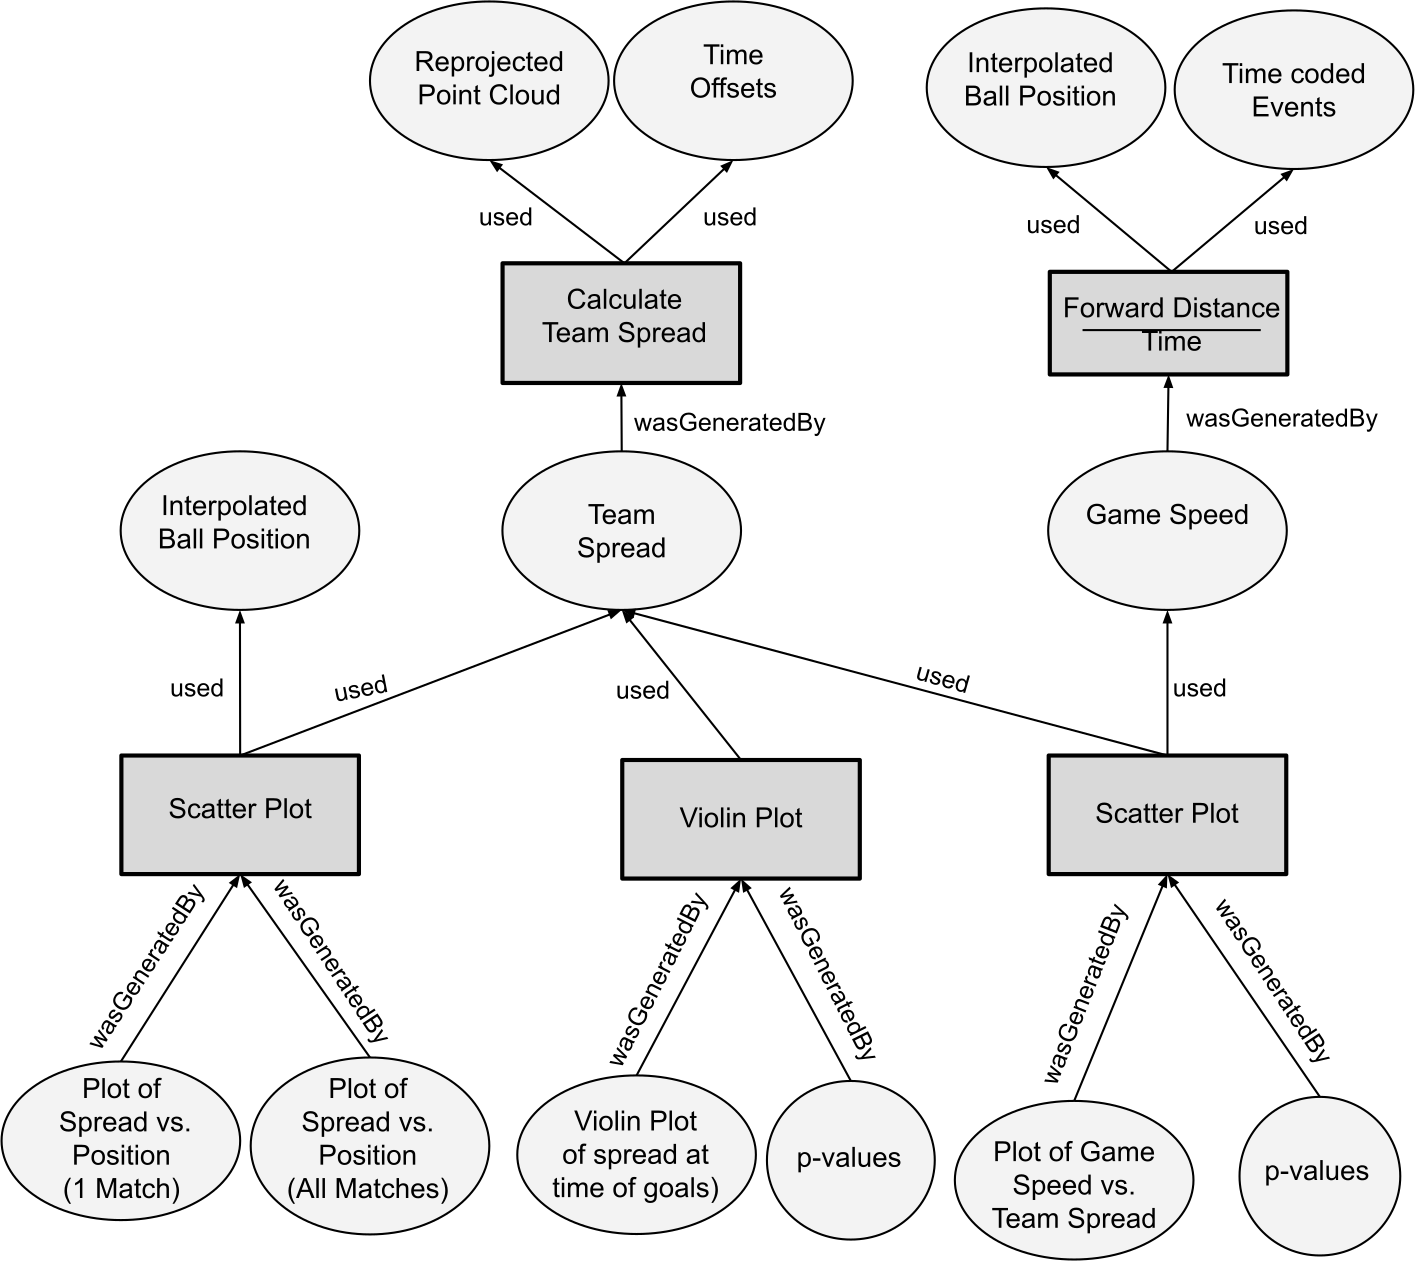
\includegraphics[width=\linewidth]{figs/prov/prov-analysis.png}
\caption{Provenance of analysis outputs in this thesis \notationdetails{}
\label{fig:prov-analysis}}
\end{figure}

To facilitate further analysis, features such as team spread and game speed were derived from the dataset. These will be discussed in depth within \secref{sec:shapepaper}. See \figref{fig:prov-analysis} for an overview of how the final analysis outputs discussed in the next section relate back to the intermediate outputs of the pipeline described in this section.
